\section{What is \BoxLib?}

\BoxLib\ is a software library containing all the functionality to write massively parallel, 
block-structured adaptive mesh refinement (AMR) applications in two and three dimensions.
\BoxLib\ is developed at the Center for Computational Sciences and Engineering (CCSE) at 
Lawrence Berkeley National Laboratory and is freely available
at {\tt https://github.com/BoxLib-Codes/BoxLib}.
The most current version of this User's Guide
can be found in the \BoxLib\ git repository at {\tt BoxLib/Docs}.  Any questions,
comments, suggestions, etc., regarding this User's Guide should be directed
to Andy Nonaka of CCSE at {\tt AJNonaka@lbl.gov}.  Further information 
about \BoxLib\ can be found by contacting Ann Almgren 
({\tt ASAlmgren@lbl.gov}) and Weiqun Zhang ({\tt WeiqunZhang@lbl.gov})
or by visiting our website, {\tt ccse.lbl.gov}.\\

If you are new to \BoxLib, we recommend you read Chapters \ref{Chap:Introduction} and
\ref{Chap:Getting Started} and familiarize yourself with the accompanying tutorial codes.
After working through Chapter \ref{Chap:Getting Started}, you will be able to run the tutorial
code on as many cores as you like!  Then, in Chapter \ref{Chap:Advanced Topics F} we enhance 
the Fortran90 tutorial code with additional features.

\section{High-Level Overview}

Key features of \BoxLib\ include:
\begin{itemize}
\item C++ and Fortran90 interfaces
\item Support for cell-centered, face-centered, edge-centered, and nodal data
\item Support for hyperbolic, parabolic, and elliptic solves on hierarchical grid structure
\item Optional subcycling in time for time-dependent PDEs
\item Supports hybrid MPI/OpenMP parallel programming model
\item Demonstrated scaling on leadership class computing facilities.
\item Plotfile format can be read by {\tt VisIt}, {\tt yt}, and {\tt AmrVis}
\item Basis of mature applications in combustion, astrophysics, cosmology, porous media, 
      and fluctuating hydrodynamics
\item Freely available at {\tt https://github.com/BoxLib-Codes/BoxLib}
\end{itemize}

\subsection{Parallel Programming Model}

The fundamental parallel abstraction in \BoxLib\ is the \MultiFab, which holds the data on the 
union of grids at a level of refinement.  A \MultiFab\ is composed of multiple ``Fortran array boxes''
(i.e., \FArrayBox es or \Fab s); each \Fab\ is a multidimensional array of data on a single grid. 
\Fab s are distributed among different processors, and
\Fab s at each level of refinement are distributed 
independently.  The software supports two data distribution schemes, as well as a 
dynamic switching scheme that decides which approach to use based on the number of 
grids at a level and the number of processors.  The first scheme is based on a 
heuristic knapsack algorithm, which emphasizes load balancing; the second is based on 
the use of a Morton-ordering space-filling curve, which emphasizes on data locality for
faster grid-to-grid communication.

\MultiFab\ operations are performed with an ``owner computes'' rule 
with each processor operating independently on its local data.  For operations that 
require data owned by other processors, the \MultiFab\ operations are preceded by a 
data exchange between processors to fill ghost cells.  Each processor contains 
meta-data that is needed 
to fully specify the data locality and processor assignments of the \Fab s. At a 
minimum, this requires the storage of an array of coordinates specifying the index space 
region for each box at each level of refinement.  The meta-data can thus be used to 
dynamically evaluate the necessary communication patterns for sharing data amongst 
processors, enabling us to optimize communications patterns within the algorithm.
By using a hybrid MPI/OpenMP approach to parallelization (see below), we are able to 
compute with fewer, larger grids, and thus the size of the meta-data is substantially 
reduced.

\subsection{Hybrid MPI--OpenMP}

The basic parallelization strategy uses a hierarchical programming approach for 
multicore architectures based on both MPI and OpenMP.  In the pure-MPI instantiation, 
each \Fab\ is assigned to a core, and each core communicates 
with every other core using only MPI.  In the hybrid approach, where multiple cores
can all access the same memory, we can assign each \Fab\ to multiple shared-memory cores,
with the work associated with that \Fab\ distributed among the cores using OpenMP.

\subsection{Parallel I/O}

Data for checkpoints and analysis are written in a self-describing format that consists 
of a directory for each time step written. Checkpoint directories contain all necessary 
data to restart the calculation from that time step. Plotfile directories contain data 
for post-processing, visualization, and analytics, which can be read using {\tt VisIt}, 
{\tt yt}, or {\tt AmrVis} (a customized visualization package developed at CCSE for 
visualizing data on AMR grids, also freely available on our website).  Within each 
checkpoint or plotfile directory is an ASCII header file and a
subdirectory for each AMR level.  The header describes the AMR hierarchy, including 
number of levels, the grids at each level, the problem size, refinement ratio 
between levels, time step, time, etc.  Each of the subdirectories contains the data 
associated with the \MultiFab\ for that level, which is stored in multiple files.
Checkpoint and plotfile directories are written at user-specified intervals.\\

Restarting a calculation can present some difficult issues for reading data efficiently. 
In the worst case, all processors would need data from all files. If multiple processors 
try to read from the same file at the same time, performance problems can result, with 
extreme cases causing file system thrashing.  Since the number of files is generally not 
equal to the number of processors and each processor may need data from multiple files, 
input during restart is coordinated to efficiently read the data. Each data file is only 
opened by one processor at a time. The {\tt IOProcessor} creates a database for mapping files 
to processors, coordinates the read queues, and interleaves reading its own data.  Each 
processor reads all data it needs from the file it currently has open.  The code tries to 
maintain the number of input streams to be equal to the number of files at all times. 
Checkpoint and plotfiles are portable to machines with a different byte ordering and 
precision from the machine that wrote the files.  Byte order and precision translations 
are done automatically, if required, when the data is read.

\subsection{Scaling}

In Figure \ref{fig:scaling} we present weak scaling results for several of our codes on 
the Cray XT5 Jaguarpf at OLCF. Jaguarpf has two hex-core sockets on each node. We assign 
one MPI process per node and spawn a single thread on each of the 12 cores. Results are 
shown for our compressible astrophysics code, {\tt CASTRO}; the low Mach number code, 
{\tt MAESTRO}; and our low Mach number combustion code, {\tt LMC}. In the {\tt MAESTRO} 
and {\tt CASTRO} tests, we simulate a full spherical star on a 3D grid with one refined 
level (2 total levels).  {\tt LMC} is tested on a 3D methane flame with detailed chemistry 
using two refined levels. {\tt MAESTRO} and {\tt LMC} scale well to 50K-100K cores, 
whereas {\tt CASTRO} scales well to over 200K cores. The overall scaling behavior 
for {\tt MAESTRO} and {\tt LMC} is not as close to ideal as that of {\tt CASTRO} 
due to the communication-intensive linear solves performed at each time step. However, 
these low Mach number codes are able to take a much larger time step than explicit 
compressible formulations in the low Mach number regime. 
%%%%%%%%%%%%%%%%%%%%%%%%%%%%%%%%%%%%%
\begin{figure}[htb]
\centering
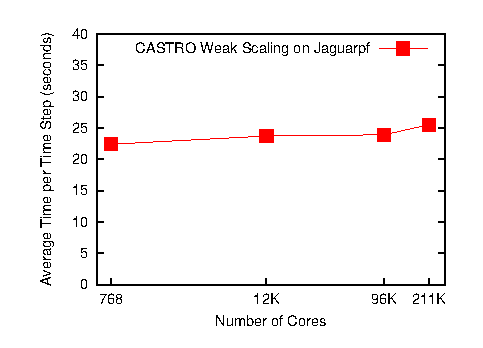
\includegraphics[width=2.1in]{./Introduction/castro_scaling}
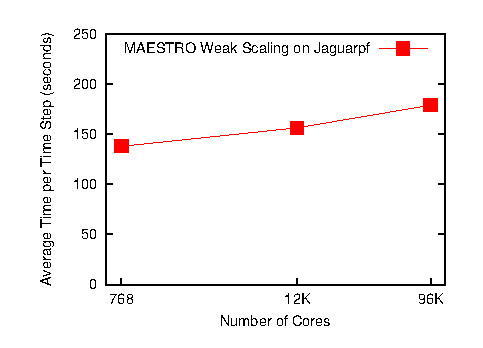
\includegraphics[width=2.1in]{./Introduction/maestro_scaling}
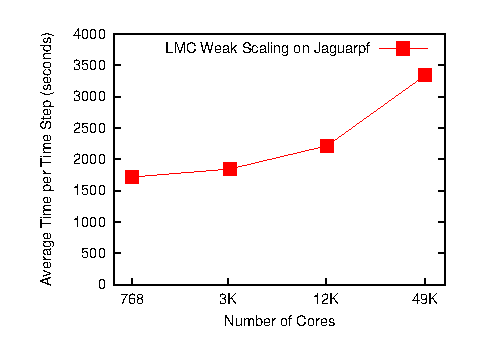
\includegraphics[width=2.1in]{./Introduction/lmc_scaling}
\caption{\label{fig:scaling}Weak scaling results for {\tt CASTRO}, {\tt MAESTRO}, and
{\tt LMC} on the Cray XT5 Jaguarpf at OLCF.}
\end{figure}
%%%%%%%%%%%%%%%%%%%%%%%%%%%%%%%%%%%%%

\section{\BoxLib\ Directory Structure}

\BoxLib\ is the base directory in a hierarchy of subdirectories that
support parallel, block-structured AMR applications in C++ and Fortran90.
A schematic of the \BoxLib\ directory structure is shown in Figure 
\ref{fig:boxlib_directory}.
%%%%%%%%%%%%%%%%%%%%%%%%%%%%%%%%%%%%%
\begin{figure}[tb]
\centering
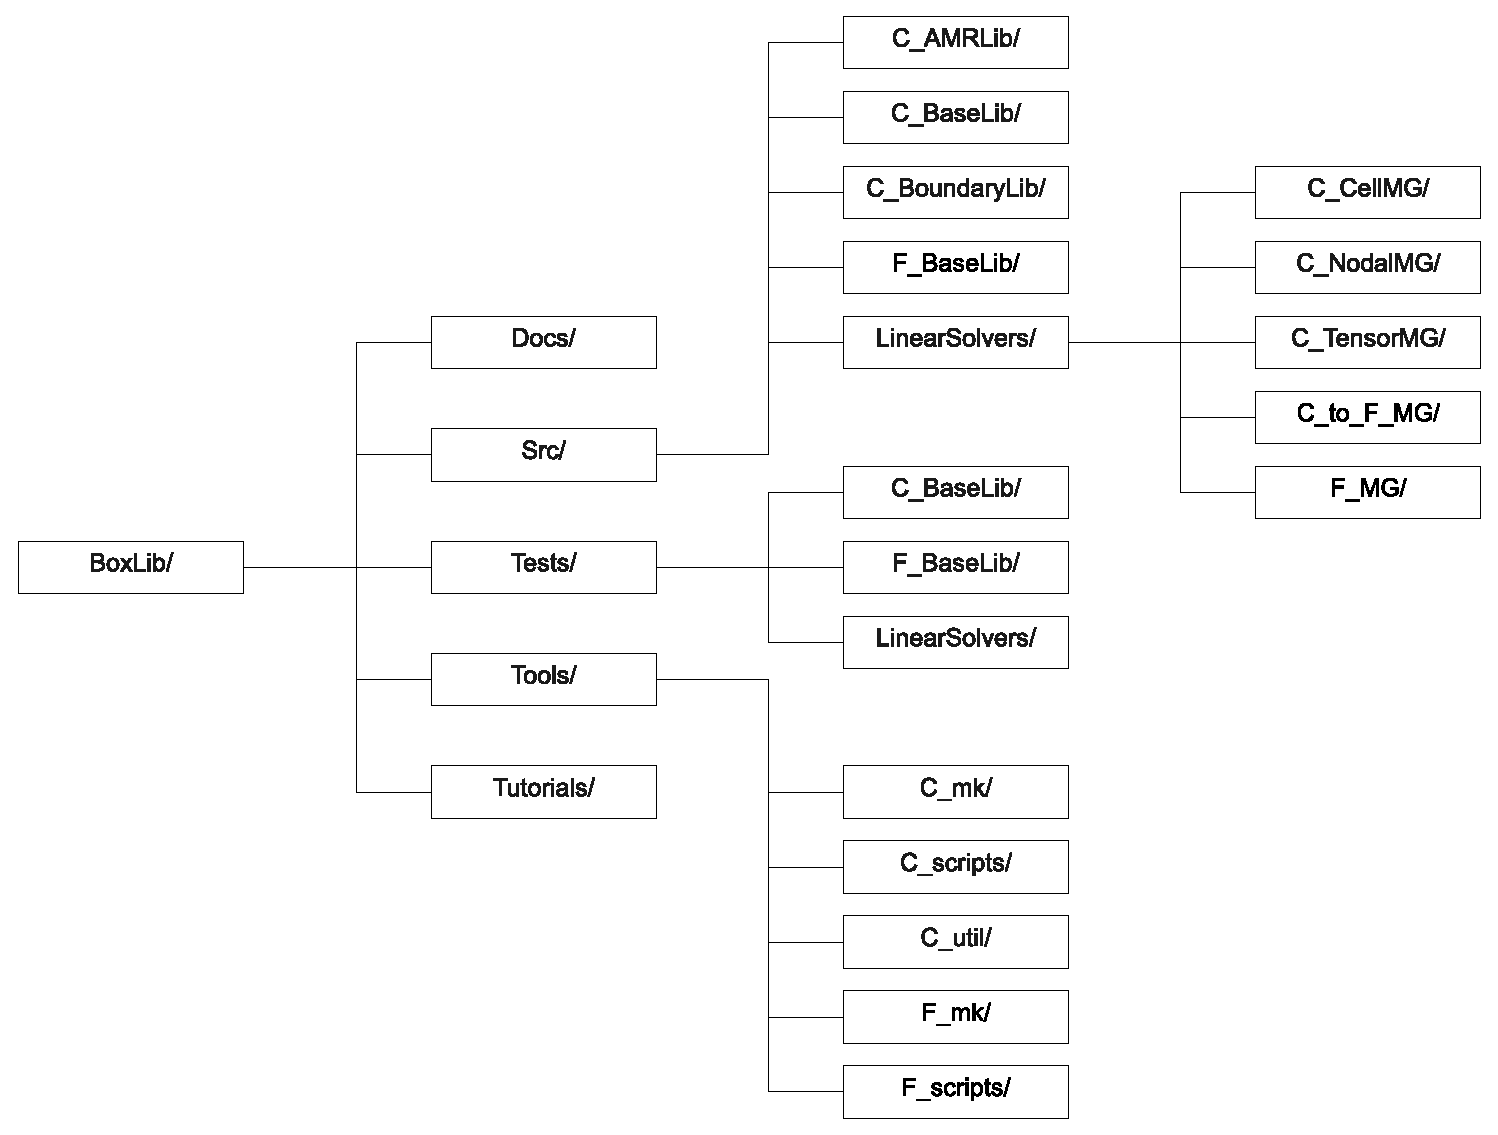
\includegraphics[width=4in]{./Introduction/boxlib_directory_bw2}
\caption{\label{fig:boxlib_directory}\BoxLib\ directory structure.}
\end{figure}
%%%%%%%%%%%%%%%%%%%%%%%%%%%%%%%%%%%%%

\begin{itemize}

\item {\tt Docs/}

Contains this \BoxLib\ User's Guide.

\item {\tt Src/}

  \BoxLib\ source code.  The C++ source code is split into several directories.
  The Fortran90 source code is contained in one directory.

  \begin{itemize}

    \item {\tt C\_BaseLib/}

    C++ base source code.

    \item {\tt C\_AMRLib/}

    C++ base source code for AMR applications.

    \item {\tt C\_BoundaryLib/}

    C++ source code for manipulating boundary data for single-level and AMR applications.

    \item {\tt F\_BaseLib/}

    Fortran90 source code.

    \item {\tt LinearSolvers/}

    Source code for various linear solvers in C++ and Fortran90.

    \begin{itemize}

      \item {\tt C\_CellMG/}
      \item {\tt C\_NodalMG/}
      \item {\tt C\_TensorMG/}
      \item {\tt C\_to\_F\_MG/}
      \item {\tt F\_MG/}

    \end{itemize}

  \end{itemize}

\item {\tt Tests/}

  Various tests used by \BoxLib\ developers.

  \begin{itemize}

  \item {\tt C\_BaseLib/}
  \item {\tt F\_BaseLib/}
  \item {\tt LinearSolvers/}

  \end{itemize}

\item {\tt Tools/}

  \begin{itemize}

  \item {\tt C\_mk/}

  The generic Makefiles that store the C++ compilation flags for
  various platforms.

  \item {\tt C\_scripts/}

  Some simple scripts that are useful for building, running,
  maintaining codes in C++.

  \item {\tt C\_Util/}

  Various utility codes for analyzing plotfiles.

  \item {\tt F\_mk/}

  The generic Makefiles that store the Fortran90 compilation flags for
  various platforms.

  \item {\tt F\_scripts/}

  Some simple scripts that are useful for building, running,
  maintaining codes in Fortran90.

  \end{itemize}

\item {\tt Tutorials/}

  Contains sample codes referred to in this User's Guide.

\end{itemize}
